%!TEX program = xelatex
\documentclass[a4paper, UTF8]{ctexrep}
\usepackage{ctex}
\usepackage{amsmath}
\usepackage{multirow}
\usepackage{amssymb}
\usepackage{graphicx}
\usepackage{geometry}
\usepackage{bm}
\usepackage{subfigure}
\usepackage{float}
\usepackage{algorithm}
\usepackage{algorithmic}

\renewcommand\thesection{\arabic{section}}

\begin{document}
	\begin{titlepage}
		\centering
		\vspace{6cm}
		\LARGE{图像处理中的数学方法第四次作业报告}\\
		\vspace{3cm}
		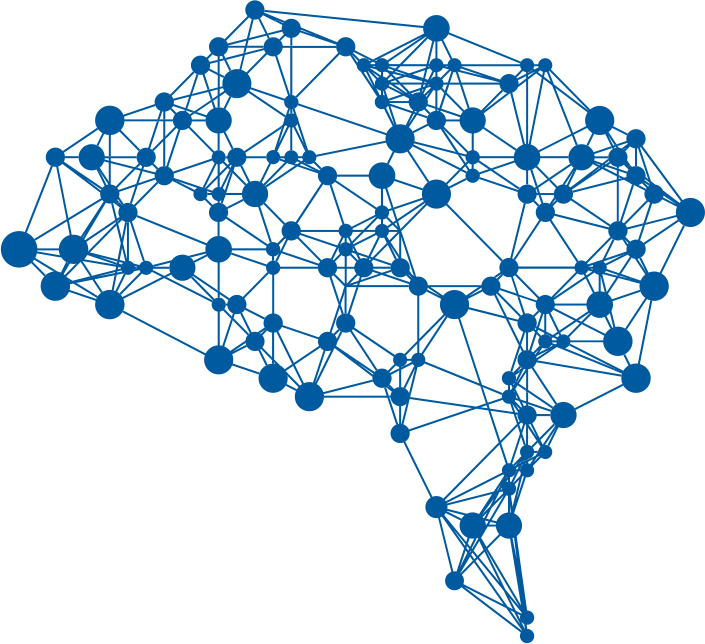
\includegraphics[width=0.8\textwidth]{deepLearning.png}\\
		\vspace{4cm}
		\normalsize{安捷 1601210097}\\
		\normalsize{\today}
	\end{titlepage}
	\section{算法描述}
		在这一次作业中,我分别实现了利用DWT算子的ADMM算法和PFBS算法,我分别用这两种算法进行了图像deblur的数值实验,现将结果报告如下。
		\subsubsection{ADMM算法流程} % (fold)
			\begin{algorithm}
				\caption{ADMM with DWT}
				\begin{algorithmic}
					\item[1] 导入图像,并对图像做进行double化,归一化,对于多通道图像进行rgb2gray,权衡计算速度调整图像大小;
					\item[2] 对图像添加模糊;
					\item[3] 算法初始化,初始化$d, b$,并预先计算迭代中需要使用的量以加快迭代速度;
					\item[4] 开始迭代,按照以下公式进行迭代$u_{k+1} = \left( A^T A + \mu I \right)^{-1} \left( A^T f + \mu W^T \left( d_k - b_k \right) \right)$
					\item[5] $d_{k+1} = \mathcal{T}_{\lambda / \mu}\left( Wu_{k+1} + b_k \right) $
					\item[6] $b_{k+1} = b_k + \delta \left( Wu_{k+1} - d_{k+1} \right)$
					\item[7] 记录误差,判断是否满足迭代终止条件,若满足则终止迭代;
					\item[8] 展示结果;
				\end{algorithmic}
			\end{algorithm}

		\subsection{PFBS算法流程}
			\begin{algorithm}
				\caption{PFBS with DWT}
				\begin{algorithmic}
					\item[1] 导入图像,并对图像做进行double化,归一化,对于多通道图像进行rgb2gray,权衡计算速度调整图像大小;
					\item[2] 对图像添加模糊;
					\item[3] 算法初始化,初始化$\alpha_0$
					\item[4] 开始迭代,按照以下公式进行迭代$g_k = \alpha_k - \nabla F_2 \left( \alpha_k \right)/L$
					\item[5] $\alpha_{k+1} = \mathcal{T}_{\lambda/L} \left( g_k \right)$
					\item[6] 直到达到最大迭代数,停止迭代;
					\item[7] 展示结果;
				\end{algorithmic}
			\end{algorithm}
		
		% subsubsection  (end)
		\subsubsection{MATLAB子函数功能说明} % (fold)
		\label{ssub:matlab子函数功能说明}
			\begin{table}[htbp!]
				\centering
				\begin{tabular}{ll}
					\hline
					函数名称 & 函数功能 \\
					\hline
					admm\_dwt.m & ADMM with DWT算法实现主脚本 \\
					gradient\_F2.m & $\nabla F_2$计算函数 \\
					PFBS\_dwt.m & PFBS with DWT算法实现主脚本 \\
					\hline
				\end{tabular}
			\end{table}
			\clearpage
		
		% subsubsection matlab子函数功能说明 (end)
		\subsubsection{参数名称及功能} % (fold)
		\label{ssub:参数名称及功能}
			\begin{table}[htbp!]
				\centering
				\begin{tabular}{llll}
					\hline
					参数名称 & 参数功能 & ADMM参数值 & PFBS参数值 \\
					\hline
					IMG\_PATH & 图像路径 &   \\
					SIGMA & 图像高斯模糊参数 & 1.5 & 1.5 \\
					NOISE\_SCALE & 图像高斯噪声参数 & 200000 & 200000\\
					MAX\_ITERATION & 最大迭代次数 & 800 & 800\\
					KERNEL\_SIZE & 图像卷积核大小 & 15 & 15 \\
					MU & ADMM算法迭代参数 & 1 &   \\
					LAMBDA & 算法迭代参数 & 0.000001 & 0.000001 \\
					TOL & ADMM终止阈值 & 1e-15 &   \\
					DELTA & ADMM迭代参数 & 0.5 &   \\
					KAPPA & PFBS迭代参数 &  &1 \\
					L & PFBS迭代参数 &  & 0.2+KAPPA \\
					FRAME & 小波框架 & 1 & 1 \\
					LEVEL & 小波分解层数 & 2 & 2 \\
					\hline
				\end{tabular}
			\end{table}
		
		% subsubsection 参数名称及功能 (end)
	\section{数值实验结果} % (fold)
		\subsection{ADMM with DWT实验结果} % (fold)
		\label{sub:admm_with_dwt实验结果}
			\begin{figure}[h]
				\centering
				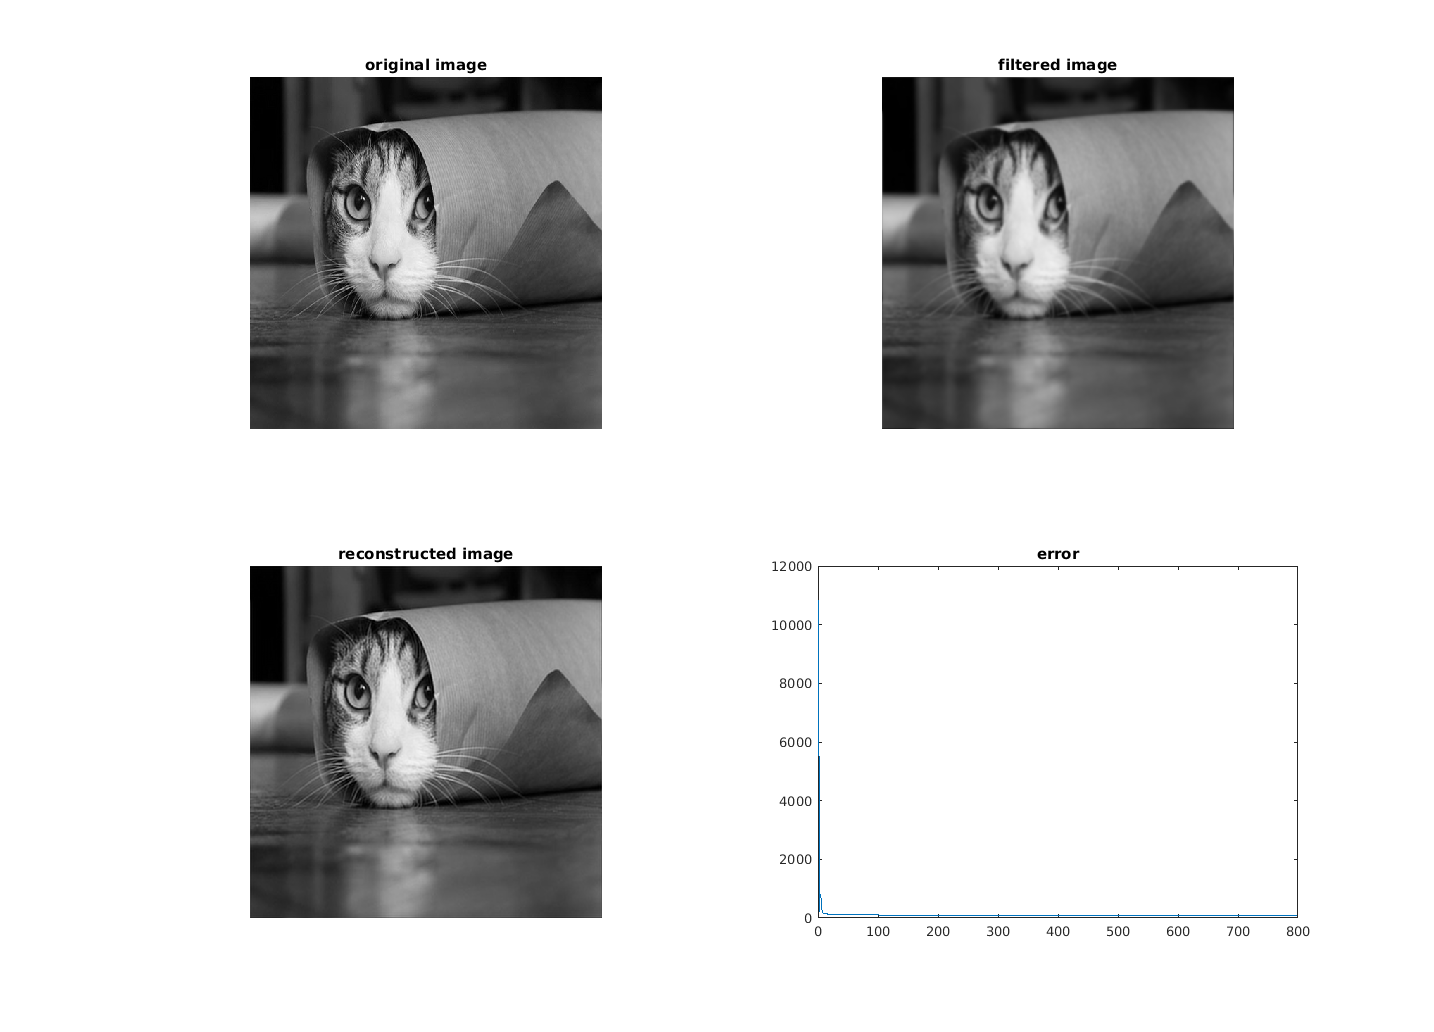
\includegraphics[width=\textwidth]{hw4_fig1.png}
				\caption{ADMM, SIGMA=1.5}
				\label{fig:figure1}
			\end{figure}
			\clearpage
			\begin{figure}[h]
				\centering
				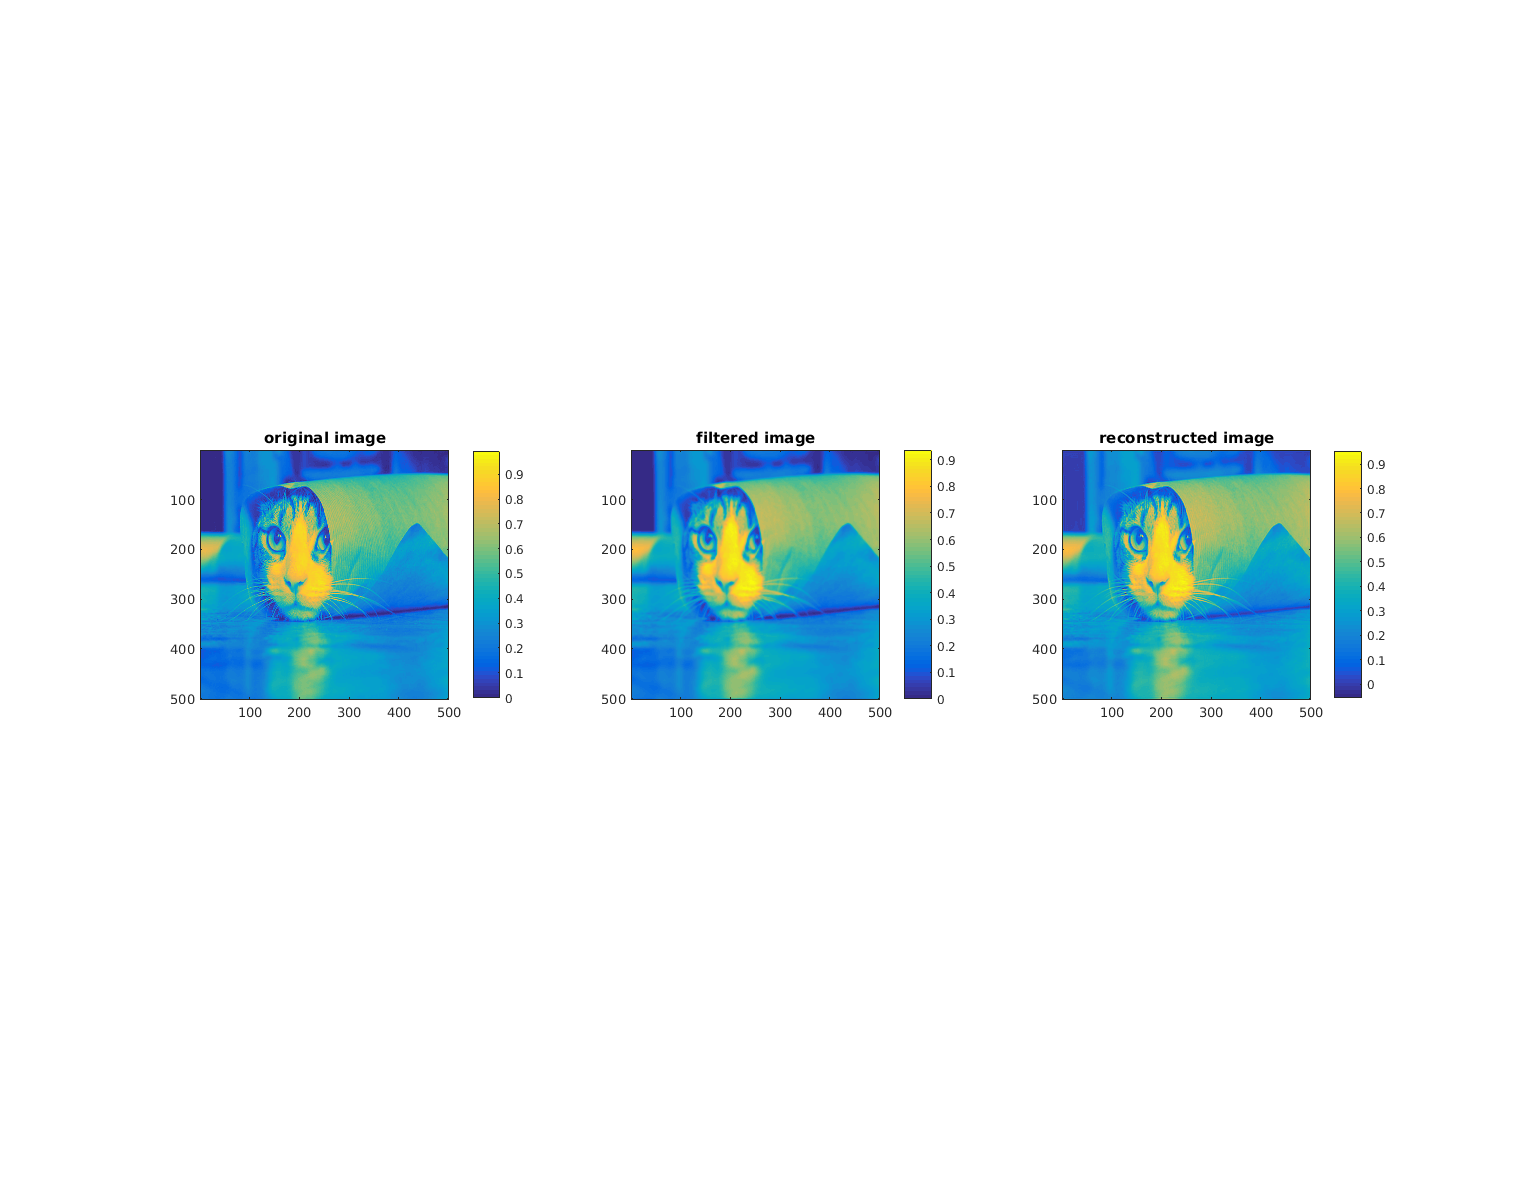
\includegraphics[width=\textwidth]{hw4_fig2.png}
				\caption{ADMM, SIGMA=1.5}
				\label{fig:figure1}
			\end{figure}
			\clearpage
			\begin{figure}[h]
				\centering
				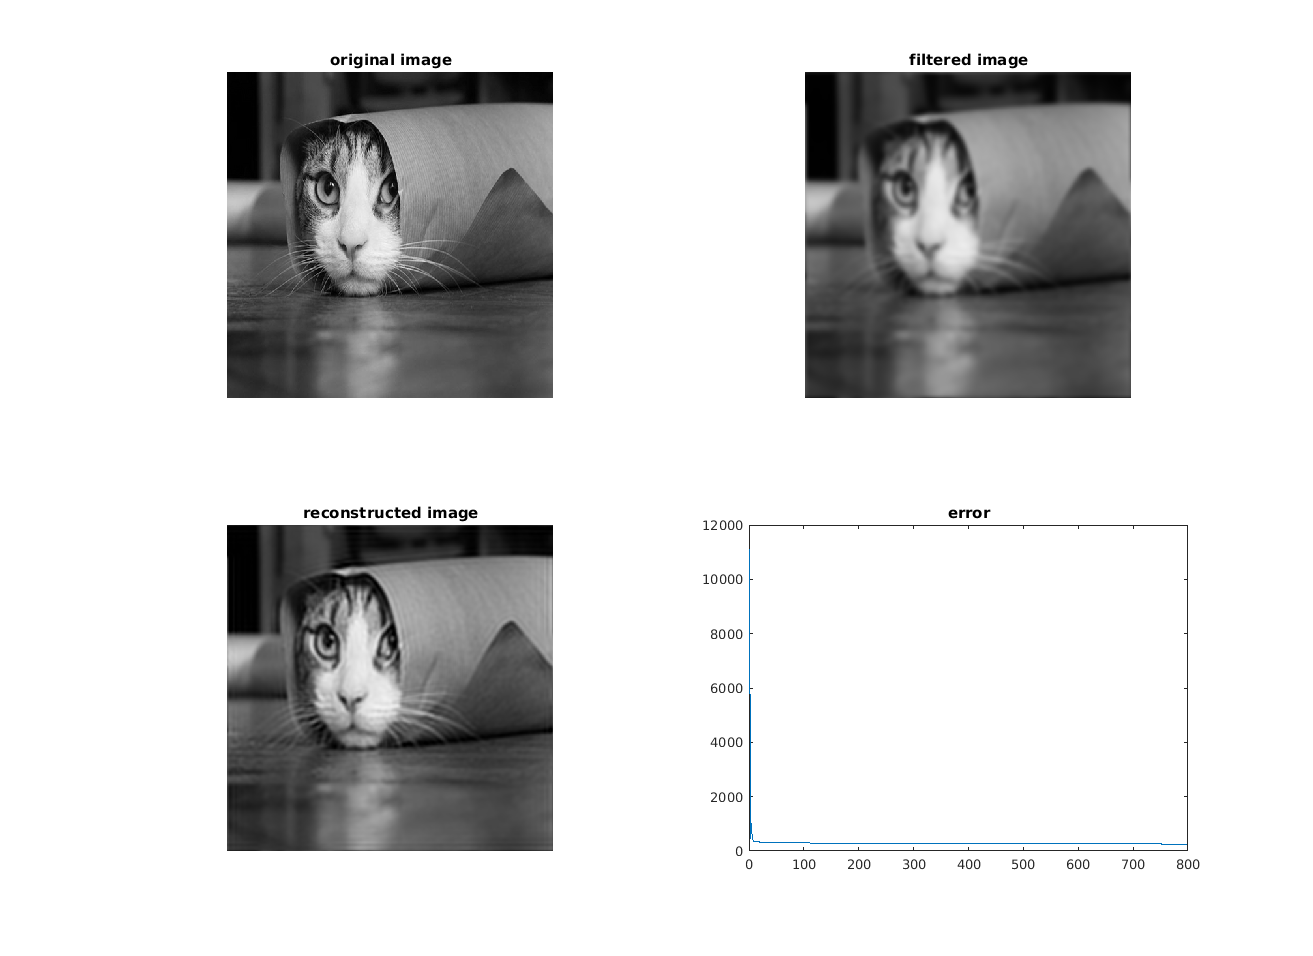
\includegraphics[width=\textwidth]{hw4_fig3.png}
				\caption{ADMM, SIGMA=3.5}
				\label{fig:figure1}
			\end{figure}
			\clearpage
			\begin{figure}[h]
				\centering
				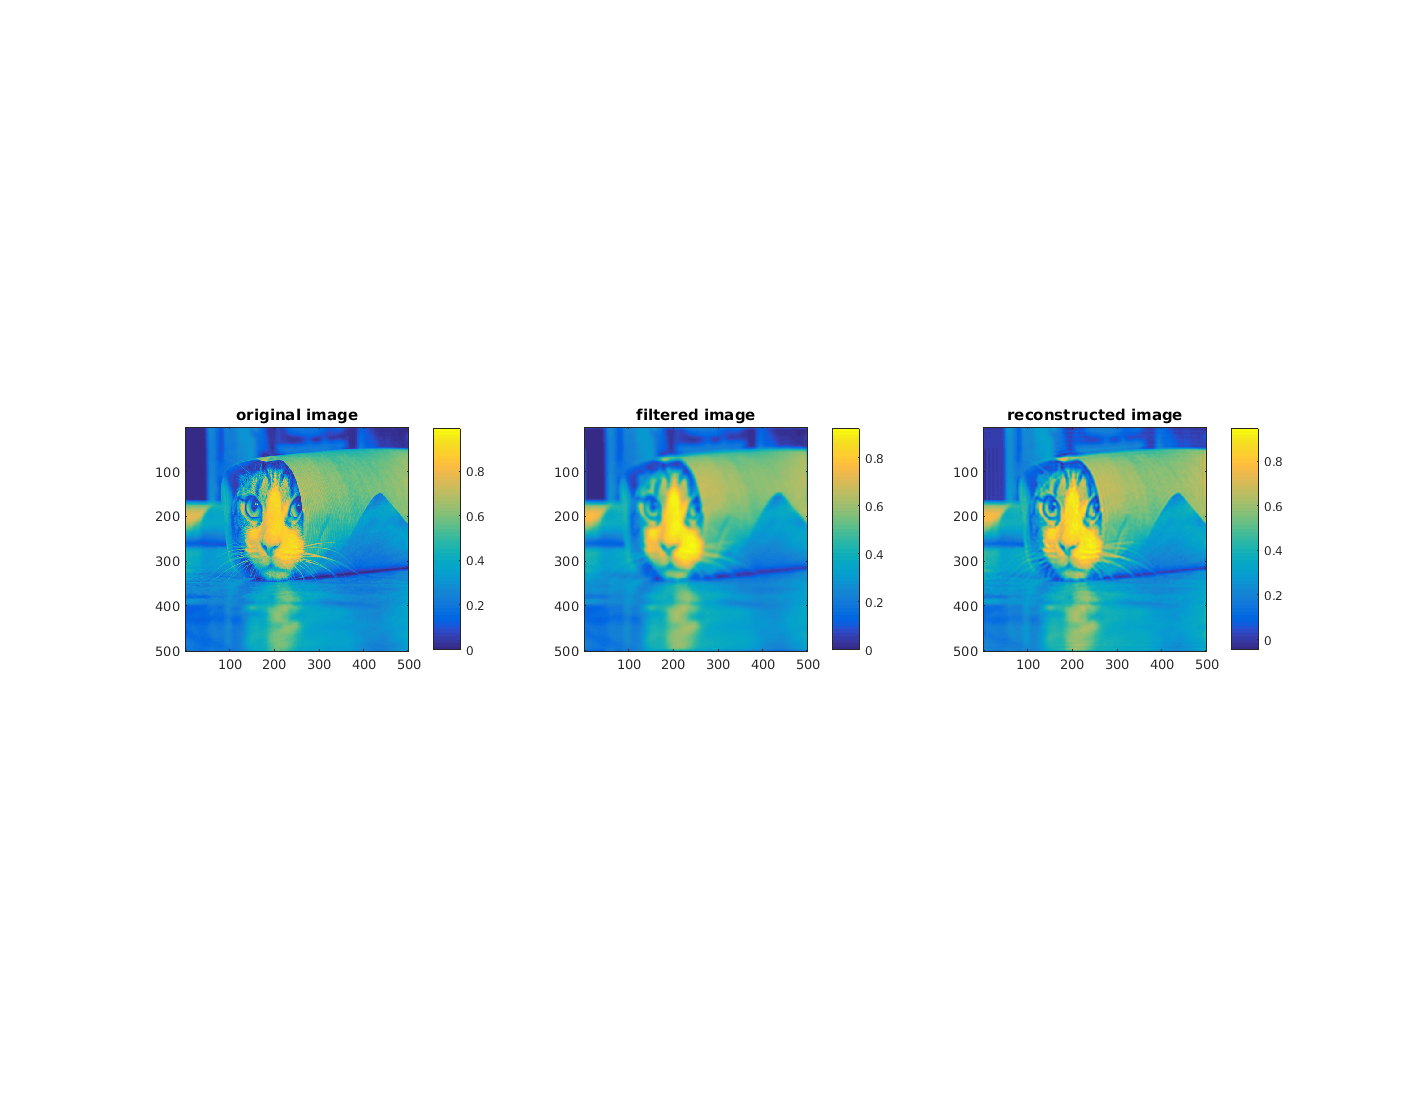
\includegraphics[width=\textwidth]{hw4_fig4.png}
				\caption{ADMM, SIGMA=3.5}
				\label{fig:figure1}
			\end{figure}
			\clearpage
			\begin{figure}[h]
				\centering
				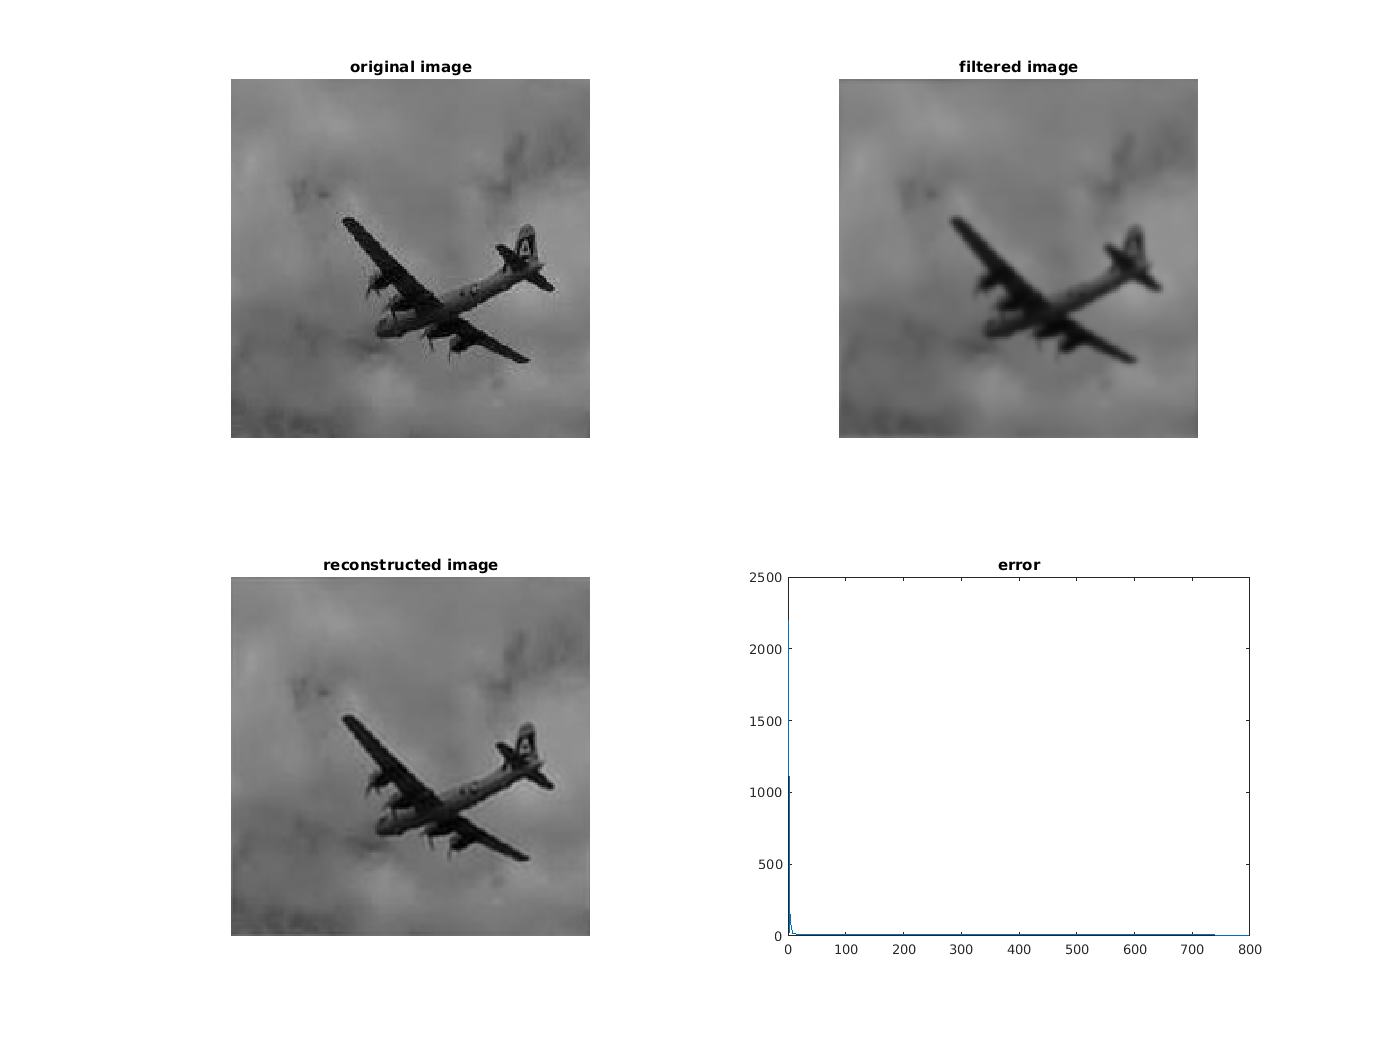
\includegraphics[width=\textwidth]{hw4_fig5.png}
				\caption{ADMM, SIGMA=1.5}
				\label{fig:figure1}
			\end{figure}
			\clearpage
			\begin{figure}[h]
				\centering
				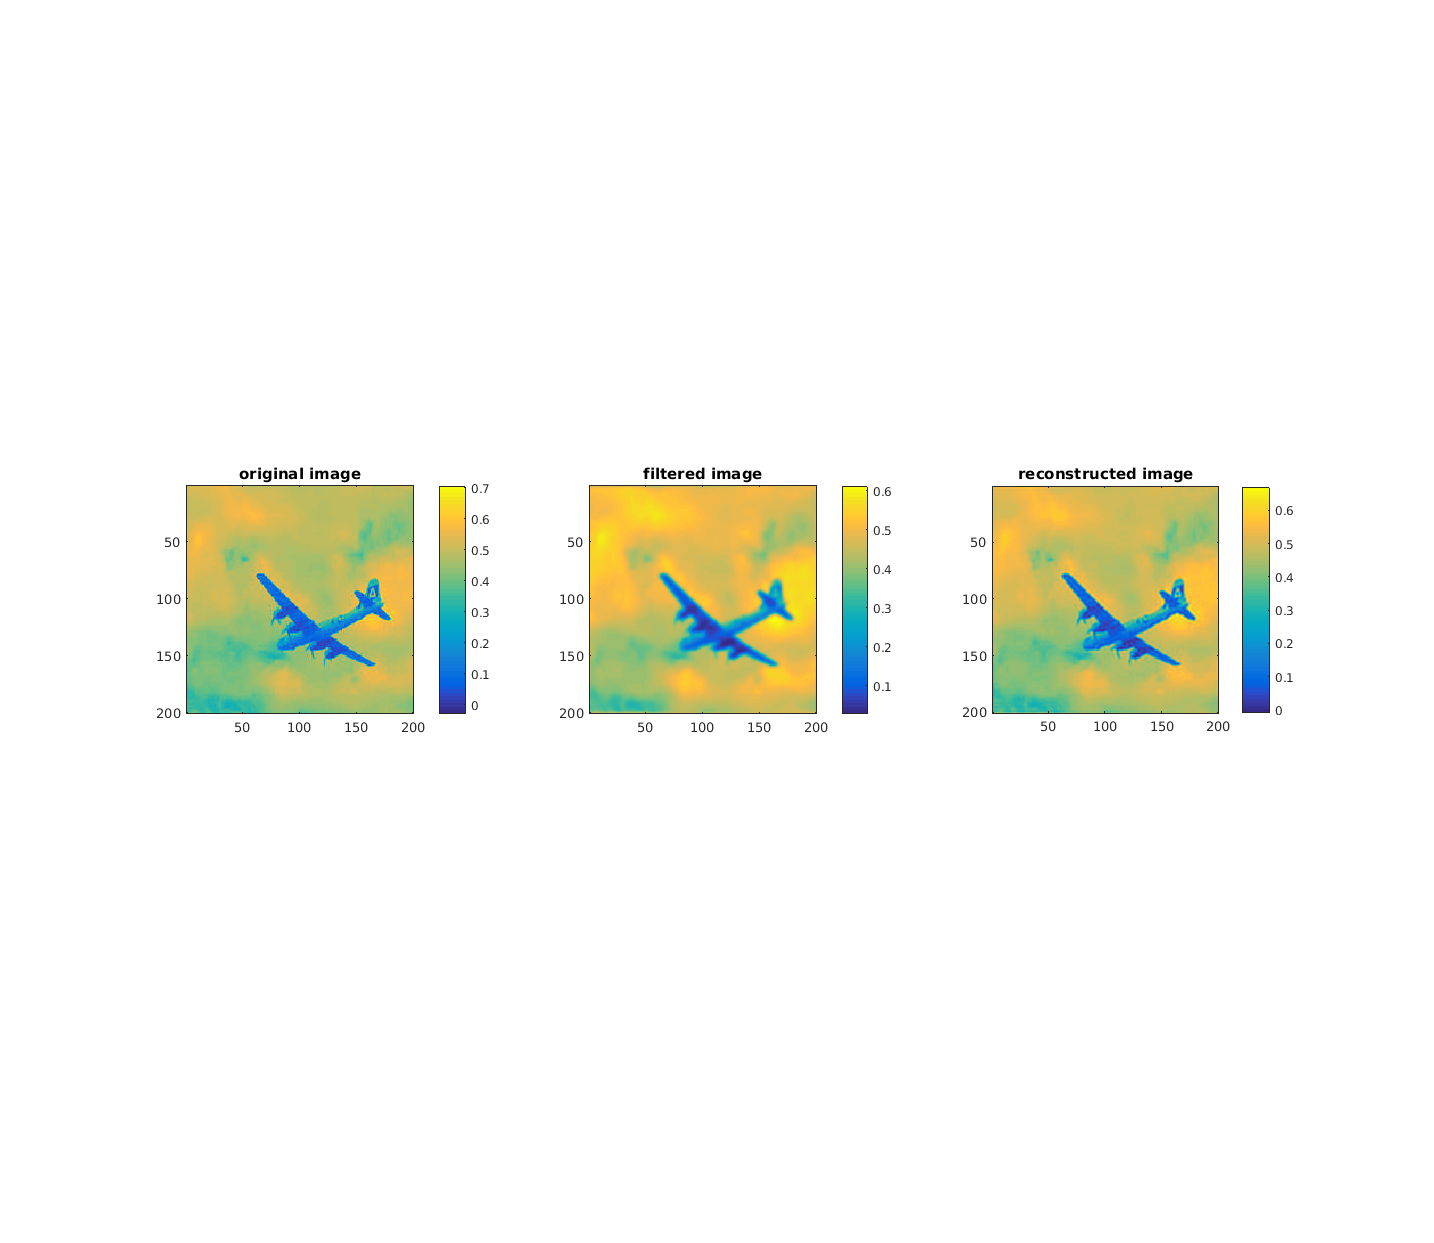
\includegraphics[width=\textwidth]{hw4_fig6.png}
				\caption{ADMM, SIGMA=1.5}
				\label{fig:figure1}
			\end{figure}
			\clearpage
		% subsection admm_with_dwt实验结果 (end)
		\subsection{PFBS with DWT实验结果} % (fold)
			\begin{figure}[h]
				\centering
				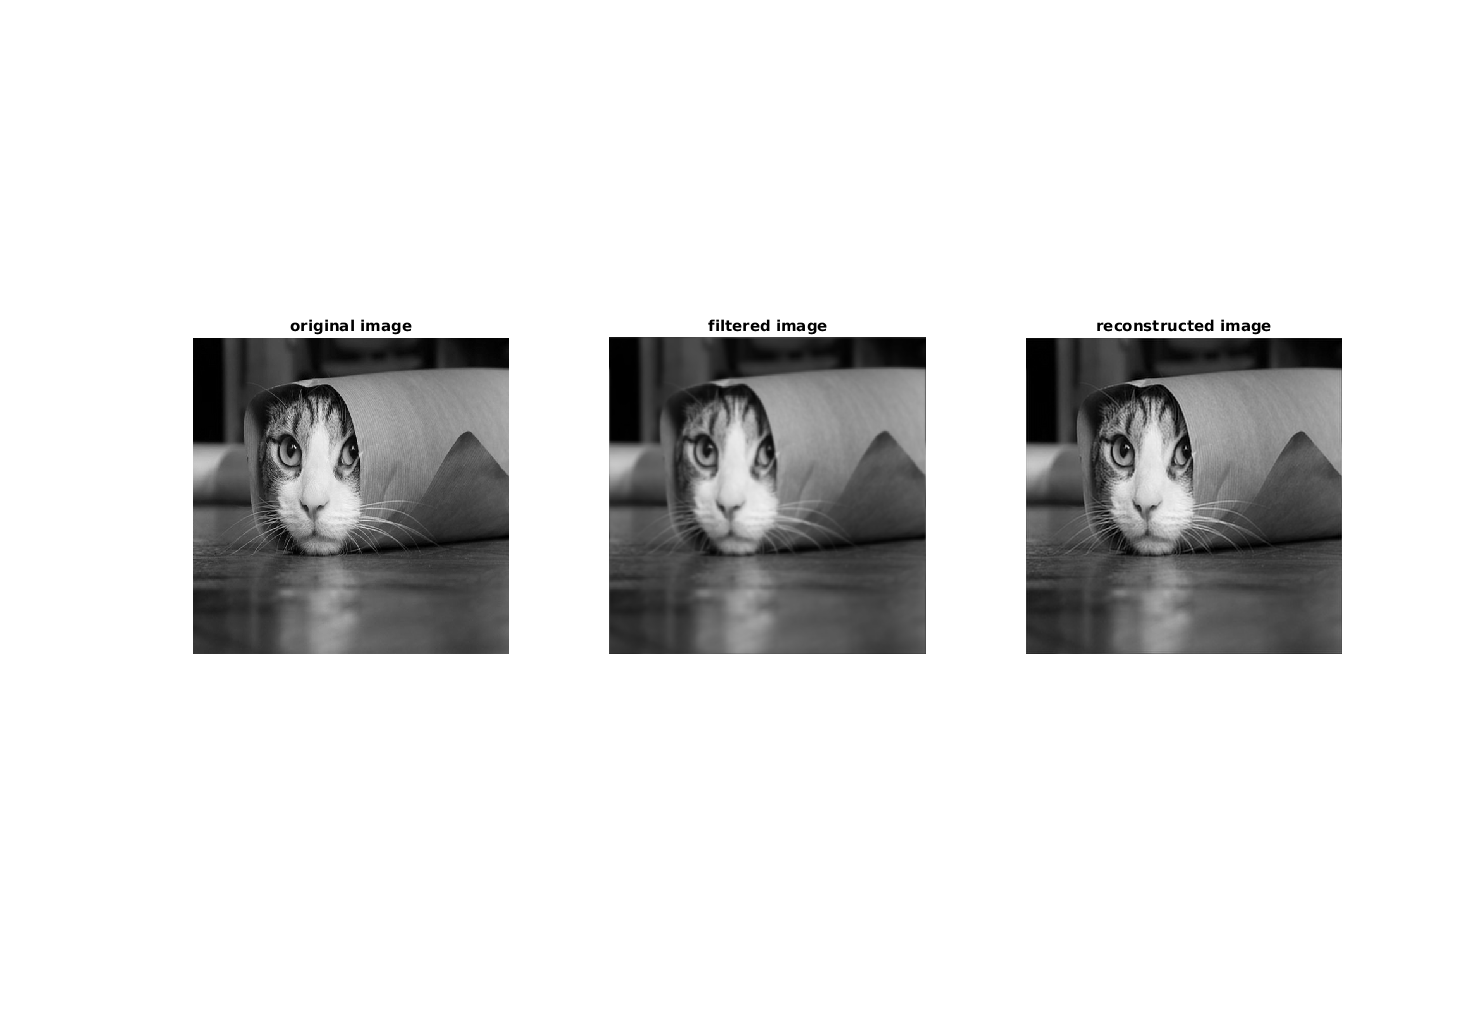
\includegraphics[width=\textwidth]{hw4_fig7.png}
				\caption{PFBS, SIGMA=1.5}
				\label{fig:figure1}
			\end{figure}
			\clearpage
			\begin{figure}[h]
				\centering
				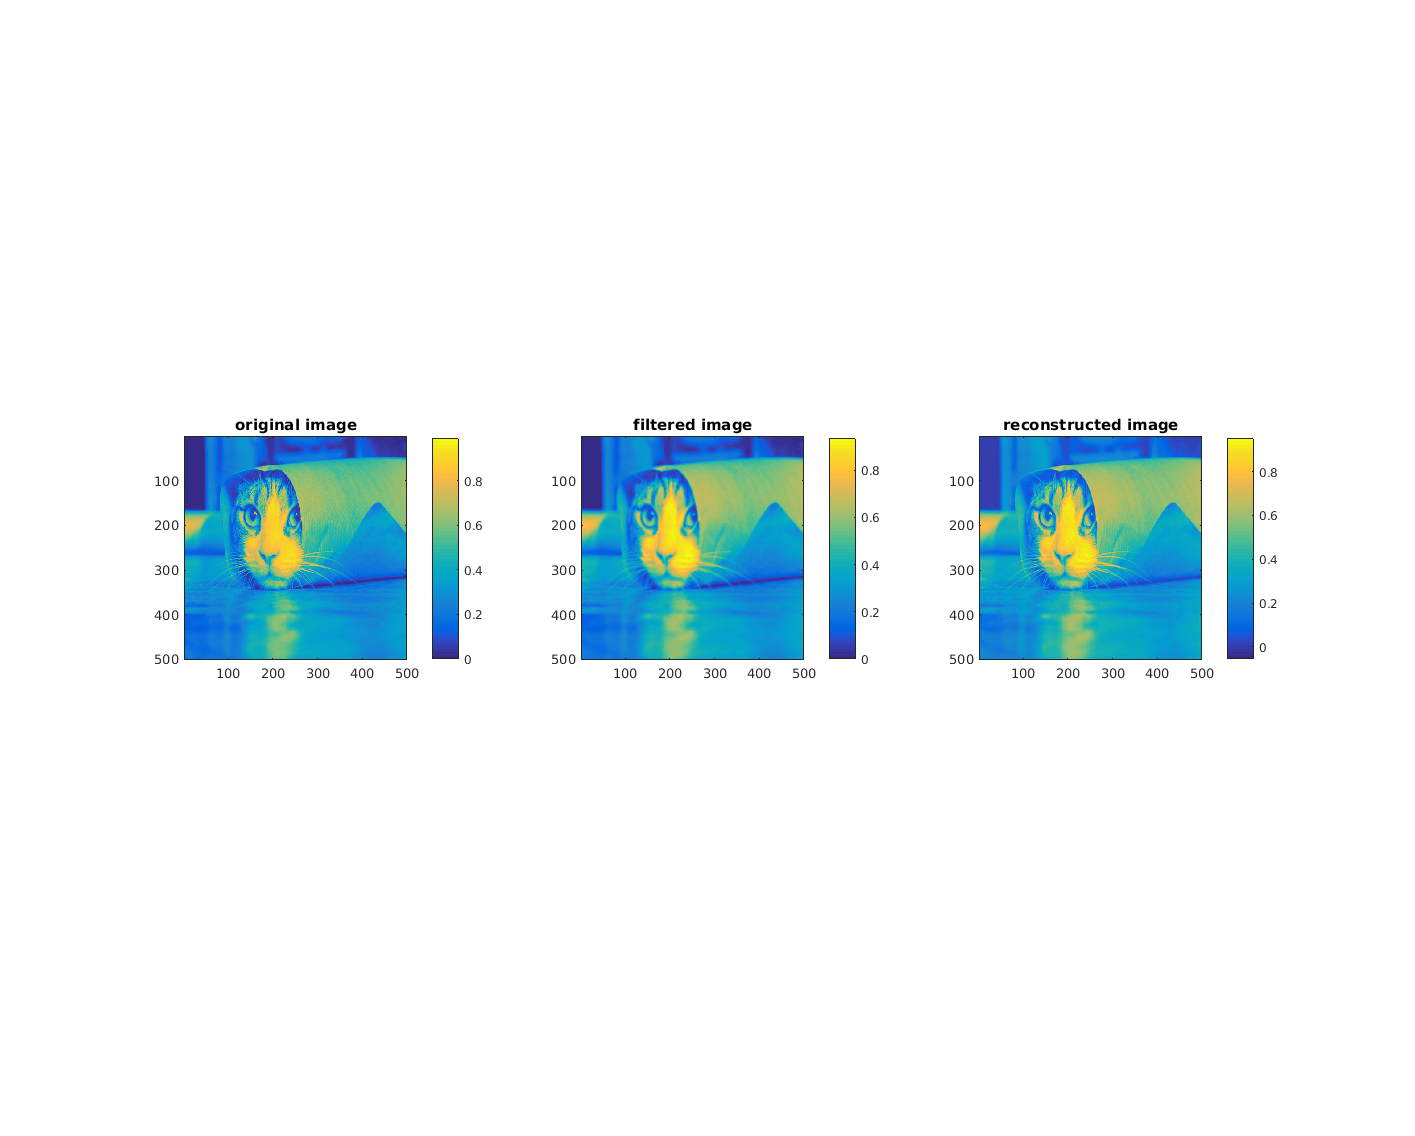
\includegraphics[width=\textwidth]{hw4_fig8.png}
				\caption{PFBS, SIGMA=1.5}
				\label{fig:figure1}
			\end{figure}
			\clearpage
			\begin{figure}[h]
				\centering
				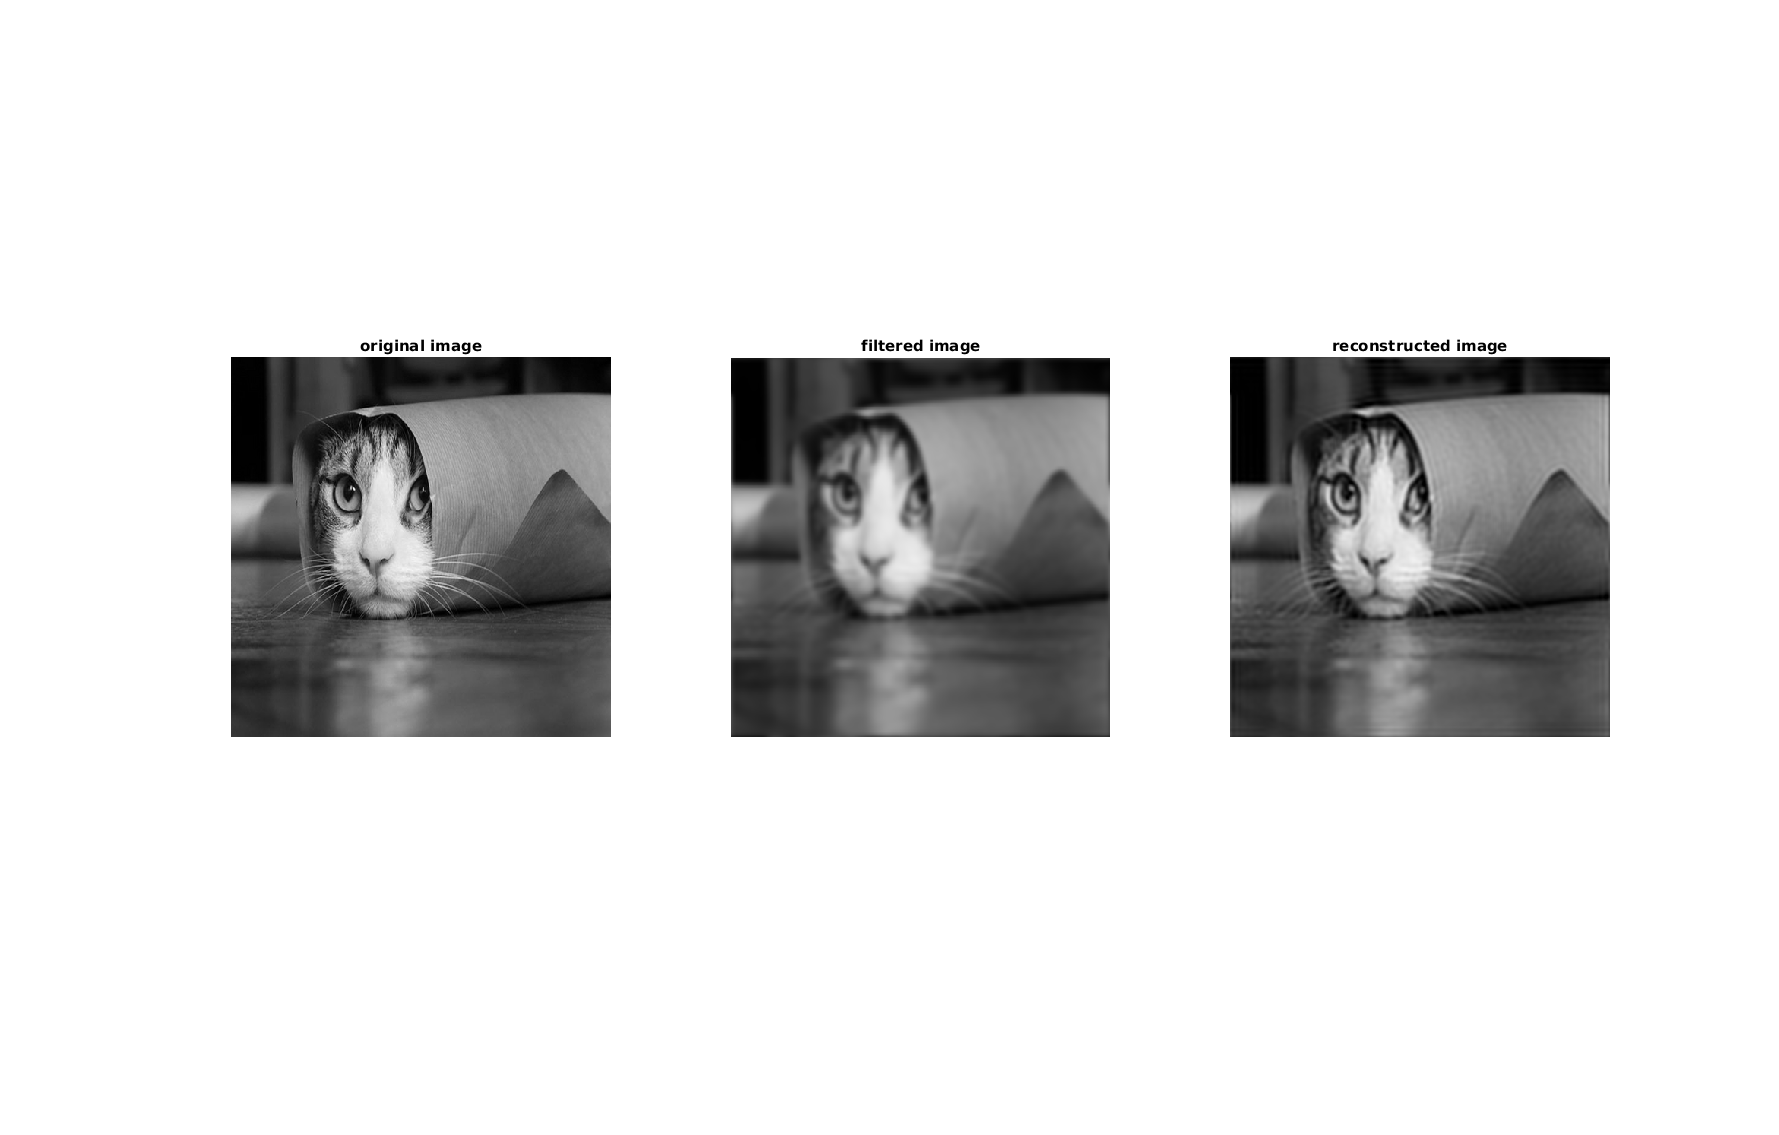
\includegraphics[width=\textwidth]{hw4_fig9.png}
				\caption{PFBS, SIGMA=3.5}
				\label{fig:figure1}
			\end{figure}
			\clearpage
			\begin{figure}[h]
				\centering
				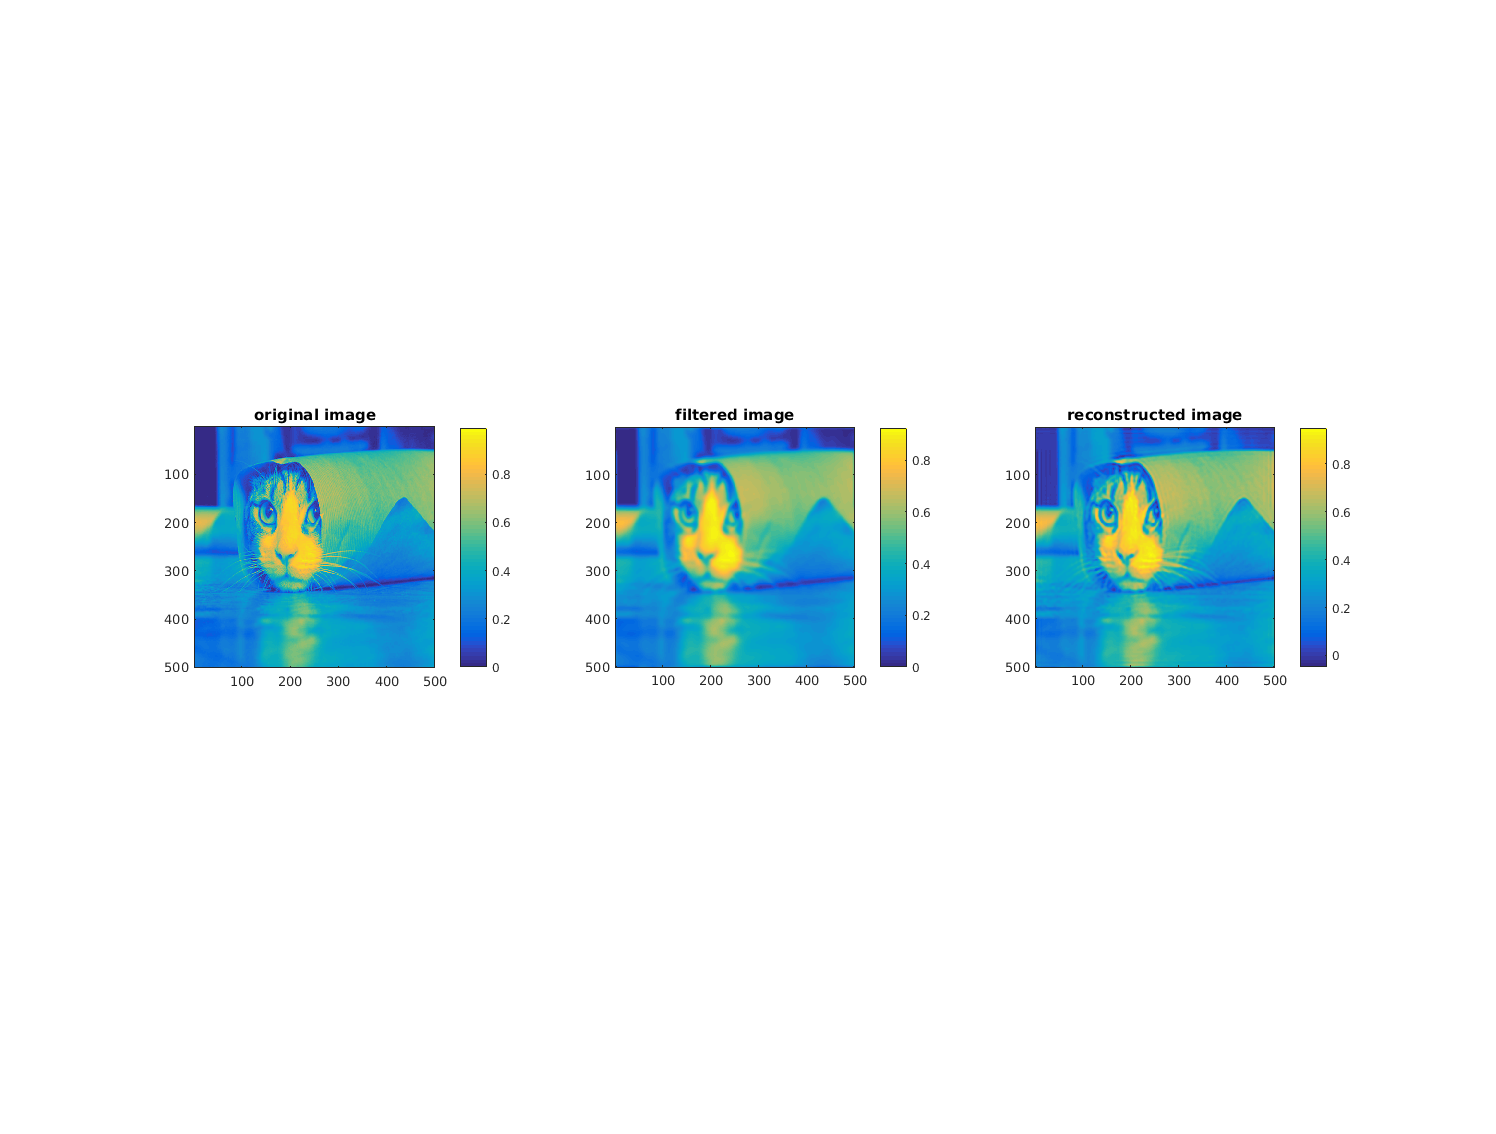
\includegraphics[width=\textwidth]{hw4_fig10.png}
				\caption{PFBS, SIGMA=3.5}
				\label{fig:figure1}
			\end{figure}
			\clearpage
			\begin{figure}[h]
				\centering
				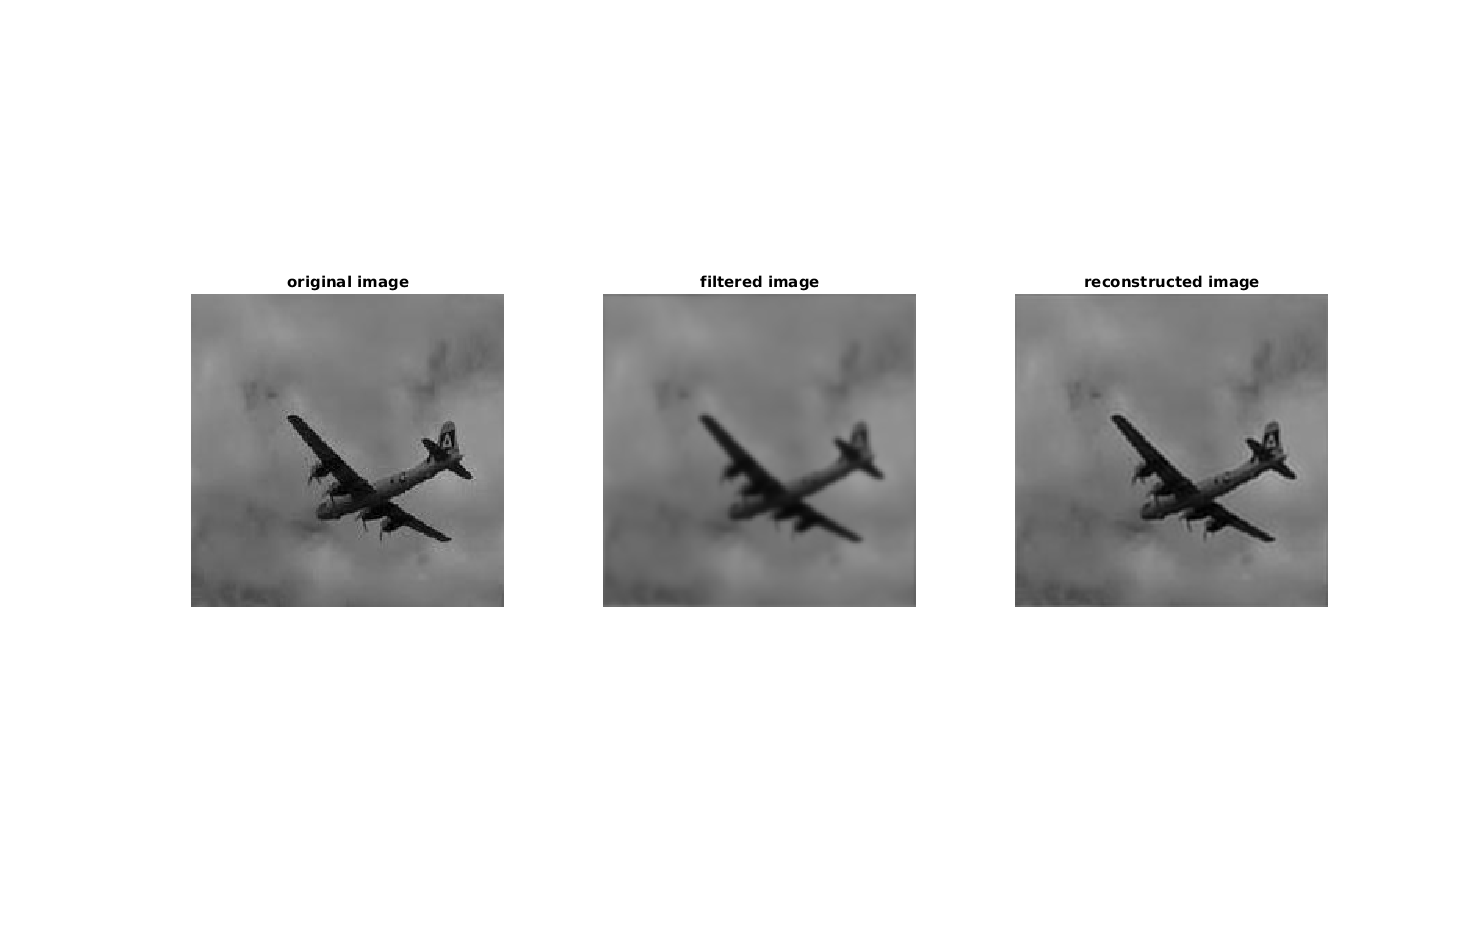
\includegraphics[width=\textwidth]{hw4_fig11.png}
				\caption{PFBS, SIGMA=1.5}
				\label{fig:figure1}
			\end{figure}
			\clearpage
			\begin{figure}[h]
				\centering
				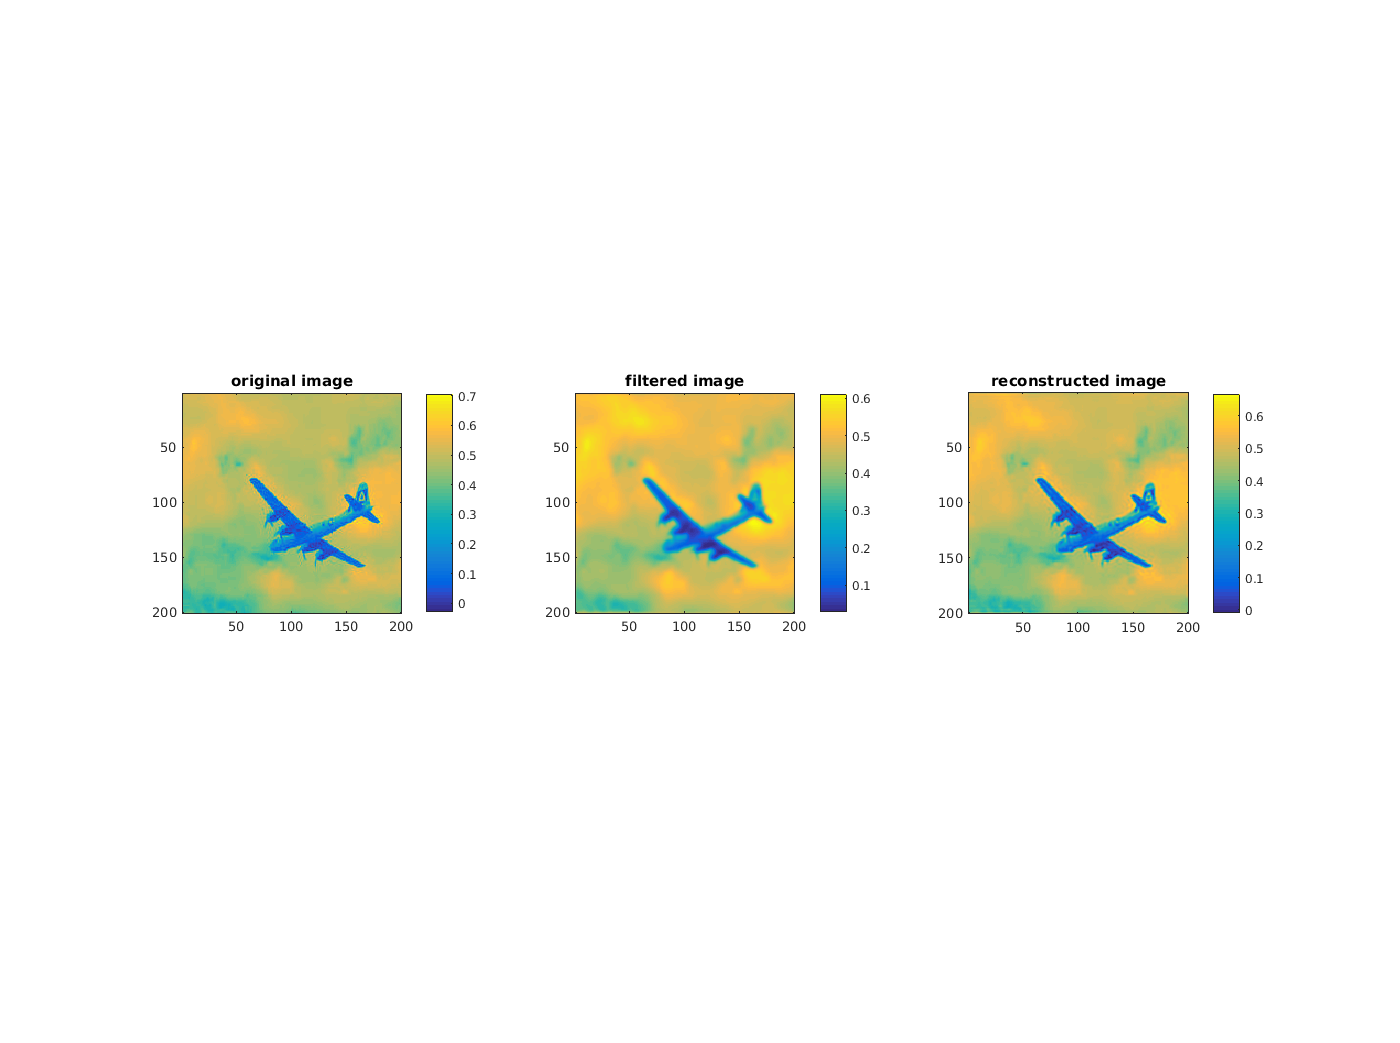
\includegraphics[width=\textwidth]{hw4_fig12.png}
				\caption{PFBS, SIGMA=1.5}
				\label{fig:figure1}
			\end{figure}
			\clearpage

	\section{总结} % (fold)
	\label{sec:总结}
		\begin{enumerate}
			\item ADMM算法与PFBS算法在使用DWT算子的情况下都可以实现一定的deblur效果;
			\item 在blur较轻的情况下,ADMM算法与PFBS算法的效果相当,blur较重时,PFBS算法的效果略优于ADMM算法;
			\item ADMM算法在使用DWT算子的情况下,deblur可以保留较多的细节,但是边缘不够锐利,在使用TV算子的情况下,可以有更锐利的边缘,但是细节损失更为严重,二者在观感上各有利弊,总体而言,DWT算子的效果更为趋真,尤其是在blur较小的情况下几乎可以完美的恢复原图像;
		\end{enumerate}
	% section 总结 (end)

	    

\end{document}